\section{Autoinducer analogues}

\subsection{Synthesis of the HHQ derivative}

The synthesis of HHQ analogue \compound{cmpd:azHHQ} is shown in \ref{sch:azHHQ_synth} and follows a route devised by Baker\cite{Baker2015}. Octonyl chloride \compound{cmpd:OctoCl} was be converted to $\beta$-ketoester \compound{cmpd:bke} via a Meldrum's acid adduct\cite{Baker2012,Scribner1978}. The $\beta$-ketoester \compound{cmpd:bke} was condensed with \textit{N}-Boc-\textit{p}-phenylenediamine \compound{cmpd:ambenboc} to form enamine \compound{cmpd:Bocenaman}. The disappointing yield of this step was in part due to the reaction proceeding to an equilibrium state rather than to completion, and hence not all of the starting material being consumed. Starting materials can be recycled to improve the yield. Alternatively, Baker later found a higher-yielding reaction using a \ce{ZrCl4} catalyst.

The enamine \compound{cmpd:Bocenaman} was cyclised with polyphosphoric acid to form amino-HHQ \compound{cmpd:amHHQ} in good yield. The amine group of amino-HHQ \compound{cmpd:amHHQ} was converted to a diazo group by reaction with \ce{NaNO2} and HCl, followed by displacement with \ce{NaN3} to form the final azido-HHQ product \compound{cmpd:azHHQ}\cite{Xu2013}.

\begin{scheme}[H]
	\begin{center}
		\schemeref[Mel]{cmpd:Mel}
		\schemeref[OctoCl]{cmpd:OctoCl}
		\schemeref[bke]{cmpd:bke}
		\schemeref[bket]{cmpd:bket}
		\schemeref[ambenboc]{cmpd:ambenboc}
		\schemeref[Bocenaman]{cmpd:Bocenaman}
		\schemeref[amHHQ]{cmpd:amHHQ}
		\schemeref[azHHQ]{cmpd:azHHQ}
		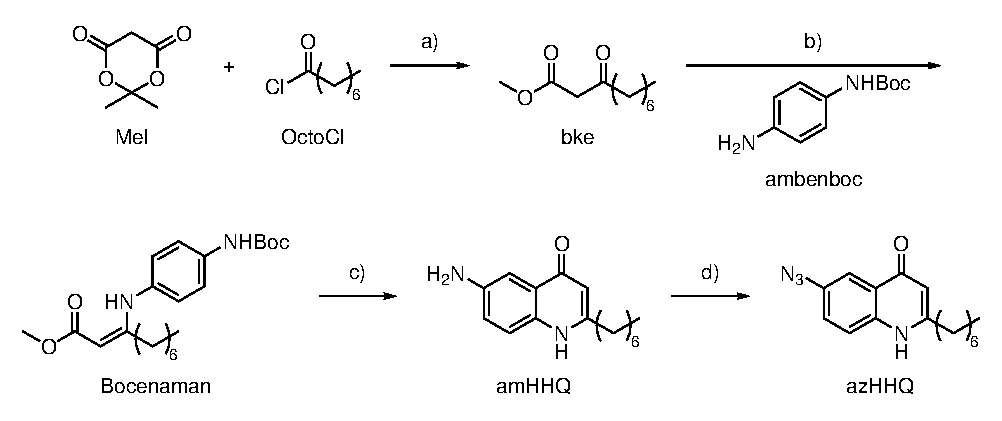
\includegraphics[scale=1]{azHHQ_synth}
		\caption{The synthesis of \compound{cmpd:azHHQ}. 
		a) i) Pyridine, DCM, $0 ^{\circ}$C. ii) MeOH, reflux, 66 \% over two steps. 
		b) MeOH, reflux, 19 \%. 
		c) Polyphosphoric acid, $120 ^{\circ}$C, 72 \%. 
		d) i) \ce{NaNO2}, HCl, \ce{H2O}, 0 $^{\circ}$C. ii) \ce{NaN3}, \ce{H2O}, r.t., 46.5 \%.
		\label{sch:azHHQ_synth}}
	\end{center}
\end{scheme}

%\subsubsection{Retrosynthesis of PQS derivative \compound{cmpd:azPQS}}
%
%The retrosynthesis of PQS analogue \compound{cmpd:azPQS} is shown in \ref{sch:azPQS_retro}. The synthesis of 1-chlorononan-2-one \compound{cmpd:Clnon} from heptyl magnesium bromide \compound{cmpd:hepGr}\cite{Hodgkinson2012} and the Weinreb amide \compound{cmpd:ClWa}\cite{Hodgkinson2011} prepared from chloroacetyl chloride \compound{cmpd:ClAcCl} has been previously described by Hodgkinson \textit{et al.}\cite{Hodgkinson2012}. 
%The synthesis of PQS described by Hodgkinson \textit{et al.}\cite{Hodgkinson2012} uses a microwave reaction of 1-chlorononan-2-one \compound{cmpd:Clnon} with anthranillic acid. It was hoped that the azide group could be installed by using 5-nitroanthranillic acid \compound{cmpd:5naa} in the place of anthranillic acid in this microwave reaction, so that the nitro group could then be converted to an azide group via an amine. However, the microwave-catalysed reaction fails when 5-nitroanthranillic acid \compound{cmpd:5naa} is used\cite{Baker2014}. Therefore, a two step process is employed instead. Firstly, ester \compound{cmpd:5naae} is formed by S$_N$2 displacement of the chlorine atom of 1-chlorononan-2-one \compound{cmpd:Clnon} by the carboxylate group of 5-nitroanthranillic \compound{cmpd:5naa}. The ester \compound{cmpd:5naae} is then cyclised using a polyphosphoric acid-catalysed reaction developed by Hradil \textit{et al.}\cite{Hradil1999} to form nitro-PQS \compound{cmpd:NPQS}.
%The nitro group can then be hydrogenated to form amino-PQS \compound{cmpd:amPQS} followed by conversion to azido-PQS \compound{cmpd:azPQS}\cite{Xu2013}.
%
%
%\begin{scheme}[H]
%	\begin{center}
%		\schemeref[hepBr]{cmpd:hepBr}
%		\schemeref[hepGr]{cmpd:hepGr}
%		\schemeref[ClAcCl]{cmpd:ClAcCl}
%		\schemeref[ClWa]{cmpd:ClWa}
%		\schemeref[Clnon]{cmpd:Clnon}
%		\schemeref[5naa]{cmpd:5naa}
%		\schemeref[5naae]{cmpd:5naae}
%		\schemeref[NPQS]{cmpd:NPQS}
%		\schemeref[amPQS]{cmpd:amPQS}
%		\schemeref[azPQS]{cmpd:azPQS}
%		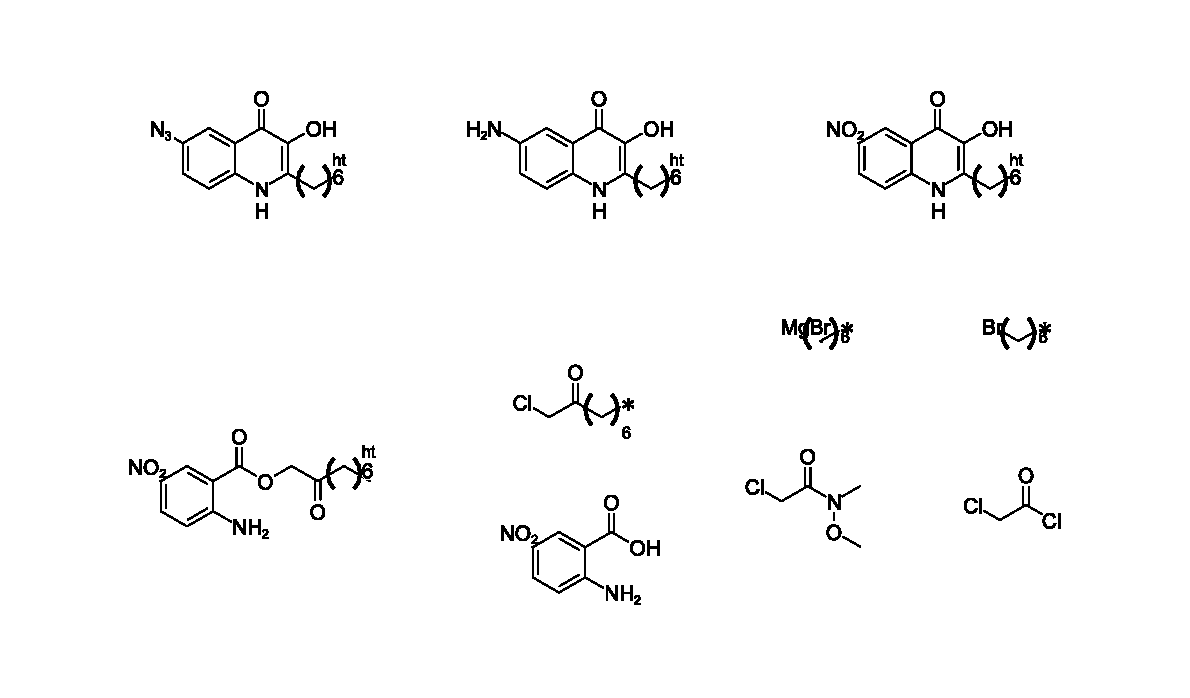
\includegraphics[scale=1]{azPQS_retro}
%		\caption{The retrosynthesis of PQS analogue \compound{cmpd:azPQS}. \label{sch:azPQS_retro}}
%	\end{center}
%\end{scheme}

\subsection{Synthesis of PQS derivative \compound{cmpd:azPQS}}

The synthesis of PQS analogue \compound{cmpd:azPQS} is shown in \ref{sch:azPQS_synth}, and also follows a route devised by Baker\cite{Baker2015}.The Weinreb amide \compound{cmpd:ClWa}\cite{Hodgkinson2011} was prepared from chloroacetyl chloride, followed by attack with heptyl magnesium bromide \compound{cmpd:hepGr} to form 1-chlorononan-2-one \compound{cmpd:Clnon} following a procedure described by Hodgkinson \textit{et al.}\cite{Hodgkinson2012}. 

The synthesis of PQS described by Hodgkinson \textit{et al.}\cite{Hodgkinson2012} uses a microwave reaction of 1-chlorononan-2-one \compound{cmpd:Clnon} with anthranillic acid. It was hoped that the azide group could be installed by using 5-nitroanthranillic acid \compound{cmpd:5naa} in the place of anthranillic acid in this microwave reaction, so that the nitro group could then be converted to an azide group via an amine. However, the microwave-catalysed reaction fails when 5-nitroanthranillic acid \compound{cmpd:5naa} is used\cite{Baker2015}. Therefore, a two step process was employed instead. 

5-Nitroanthranillic acid \compound{cmpd:5naa} was heated with \ce{K2CO3} to deprotonate the carboxylic acid, followed by addition of 1-chlorononan-2-one \compound{cmpd:Clnon} to form the ester \compound{cmpd:5naae} by S$_N$2 displacement of the chlorine atom in a procedure adapted from Hlav\'a\u c et al.\cite{Hlavac2004}. Cyclisation with polyphosphoric acid produced nitro-PQS \compound{cmpd:NPQS} cleanly\cite{Hlavac2004,Hradil1999}. 

Conditions for the reduction of the nitro group were then compared (see \ref{tbl:amPQS_opt}). Baker initially used Zn and HCl, however this gave a yield over 100 \% suggesting coordination of amino-PQS \compound{cmpd:amPQS} to the Zn\cite{Baker2015}. 

Reduction with \ce{SnCl2} was attempted, but no product was detected by LCMS. Catalytic hydrogenation was then attempted. We determined that nitro-PQS \compound{cmpd:NPQS} could not be reduced using \ce{H2} and Pd/C at room temperature and pressure. However, increasing the pressure to 3 atm is sufficient to cause conversion to amino-PQS \compound{cmpd:amPQS} in 4 h. Achieving 3 atm pressure of \ce{H2} in a lab environment requires the use of a Parr hydrogenator, and it was found to be more convenient to use \ce{PtO2} as a catalyst as this allows the reaction to proceed at room pressure and temperature\cite{Shen2006a}. Finally, amino-PQS \compound{cmpd:amPQS} was converted to azido-PQS \compound{cmpd:azPQS} by reaction with \ce{NaNO2} and HCl to form diazo-PQS, followed by displacement of the diazo group using \ce{NaN3} to give the azido-PQS \compound{cmpd:azPQS}\cite{Xu2013}.

\renewcommand{\arraystretch}{1.2}
\begin{table}[ht]
  \centering
\begin{tabular}{|l|l|}
\hline 
\textbf{Conditions} & \textbf{Outcome} \\ 
\hline 
\ce{SnCl2}.2\ce{H2O}, MeOH, r.t., 18 h & No reaction \\ 
\hline 
\ce{H2}, Pd/C, MeOH, 3 atm, r.t., 4 h. & Product \compound{cmpd:amPQS}, 100 \% yield \\ 
\hline 
\ce{H2}, \ce{PtO2}, MeOH, 1 atm, r.t., 45 min & Product \compound{cmpd:amPQS}, 80 \% yield \\ 
\hline 
\end{tabular}
\caption{Conditions attempted for the synthesis of \compound{cmpd:amPQS}. \label{tbl:amPQS_opt}} 
\end{table}

\begin{scheme}[H]
	\begin{center}
		\schemeref[hepBr]{cmpd:hepBr}
		\schemeref[hepGr]{cmpd:hepGr}
		\schemeref[ClAcCl]{cmpd:ClAcCl}
		\schemeref[ClWa]{cmpd:ClWa}
		\schemeref[Clnon]{cmpd:Clnon}
		\schemeref[5naa]{cmpd:5naa}
		\schemeref[5naae]{cmpd:5naae}
		\schemeref[NPQS]{cmpd:NPQS}
		\schemeref[amPQS]{cmpd:amPQS}
		\schemeref[azPQS]{cmpd:azPQS}
		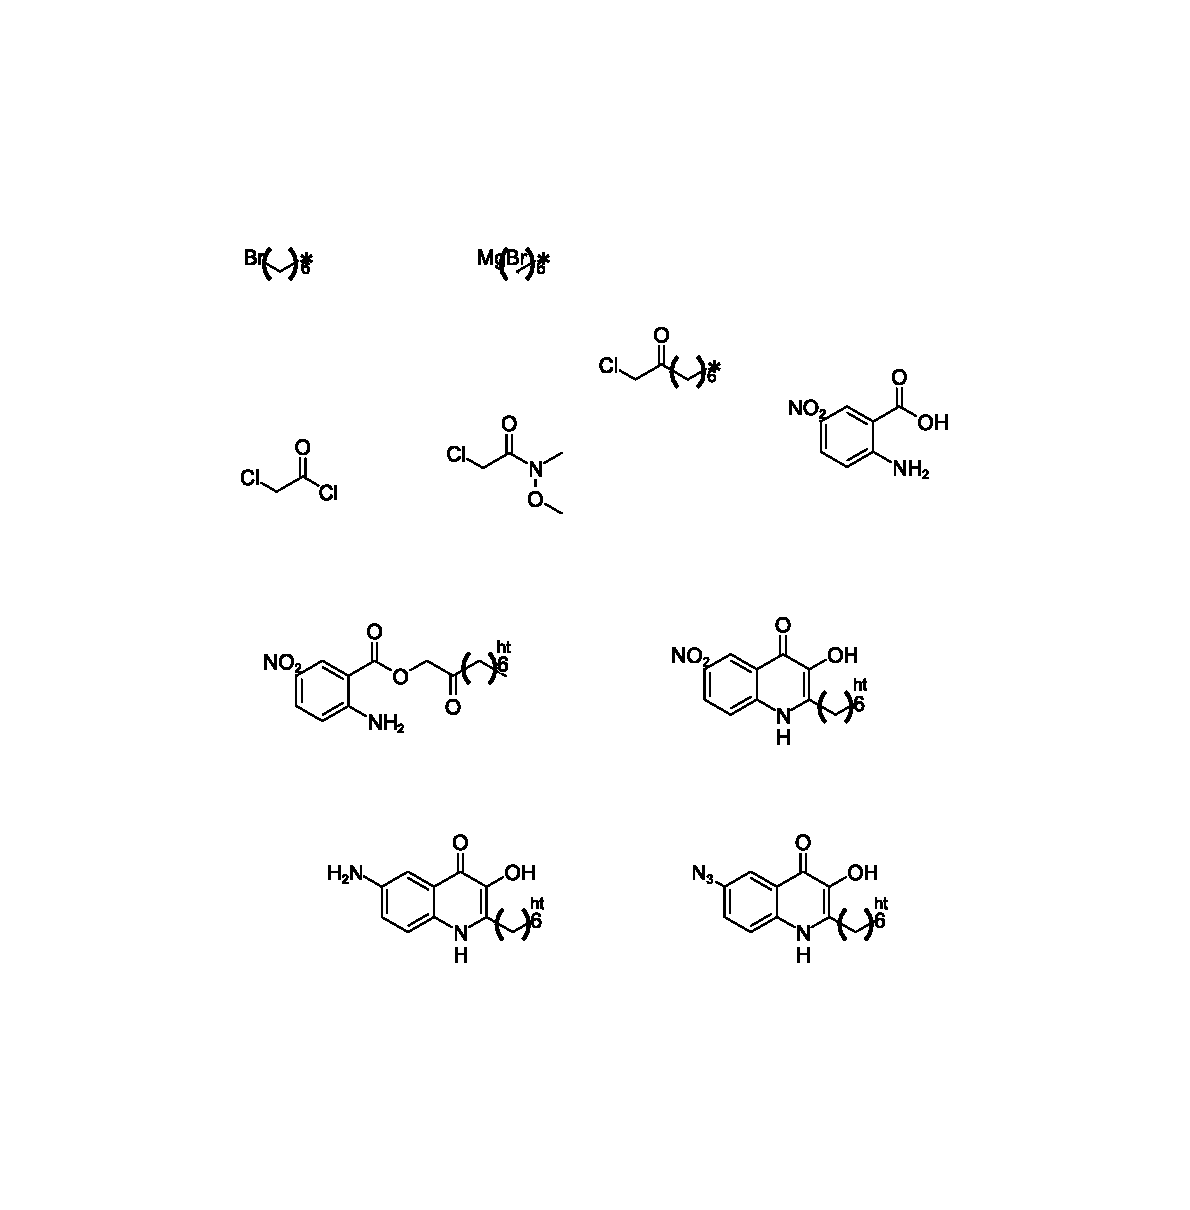
\includegraphics[scale=1]{azPQS_synth}
		\caption{The synthesis of \compound{cmpd:azPQS}.
		a) Mg turnings, THF, r.t., 2 h then reflux, 2 h.
		b) \textit{N},\textit{O}-dimethylhydroxyl amine hydrochloride, \ce{K2CO3}, toluene, \ce{H2O}, - 5 $^{\circ}$C to r.t., 30 min, 71 \%.
		c) THF, 0 $^{\circ}$C to r.t., 15 h, 96 \%.
		d) \compound{cmpd:5naa}, \ce{K2CO3}, DMF, 90 $^{\circ}$C, 1 h, then \compound{cmpd:Clnon}, r.t., 18 h, 100 \%.
		e) Polyphosphoric acid, 90 $^{\circ}$C, 5.5 h, 40 \%.
		f) \ce{H2}, \ce{PtO2}, MeOH, 1 atm, r.t., 45 min, 80 \%.
		g) i) \ce{NaNO2}, HCl, \ce{H2O}, 0 $^{\circ}$C, 50 min. ii) \ce{NaN3}, \ce{H2O}, r.t., 4 h, 28 \% over two steps.
		\label{sch:azPQS_synth}}
	\end{center}
\end{scheme}

\subsection{C$_4$-HSL derivatives}

\subsubsection{Retrosynthesis of C$_4$-HSL derivatives \compound{cmpd:HL2N3}, \compound{cmpd:HL4N3} and \compound{cmpd:HL6N3}}

The azido analogue of C$_4$-HSL with a C$_2$ chain \compound{cmpd:HL2N3} (see \ref{fig:HL_anas}) has previously been prepared by Stacey \textit{et al.} \cite{Stacy2013}. It uses the cyclisation of \textsc{l}-methionine \compound{cmpd:LM} using bromoacetic acid via the mechanism shown in \ref{sch:HLHBr_mech} to form the homoserine lactone HBr salt \compound{cmpd:HLHBr}. This is then converted by a biphasic one-pot process to the azido-C$_2$ analogue \compound{cmpd:HL2N3} using bromoacetyl bromide \compound{cmpd:Br2Br} and \ce{NaN3}. It was hoped that this procedure could also be used to produce the azido-C$_4$ and C$_6$ chain analogues.

\begin{scheme}[H]
	\begin{center}
		\schemeref[LM]{cmpd:LM}
		\schemeref[HLHBr]{cmpd:HLHBr}
		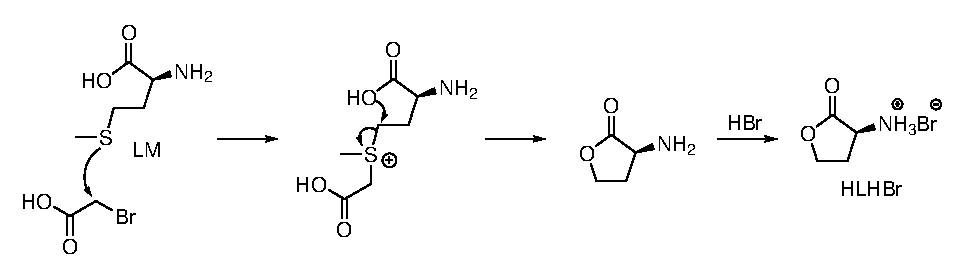
\includegraphics[scale=1]{HLHBr_mech}
		\caption{The mechanism of formation of \compound{cmpd:HLHBr}. \label{sch:HLHBr_mech}}
	\end{center}
\end{scheme}

\begin{scheme}[H]
	\begin{center}
		\schemeref[LM]{cmpd:LM}
		\schemeref[HLHBr]{cmpd:HLHBr}
		\schemeref[Br2Br]{cmpd:Br2Br}
		\schemeref[Cl4Br]{cmpd:Cl4Br}
		\schemeref[Cl6Br]{cmpd:Cl6Br}
		\schemeref[HL2N3]{cmpd:HL2N3}
		\schemeref[HL4N3]{cmpd:HL4N3}
		\schemeref[HL6N3]{cmpd:HL6N3}
		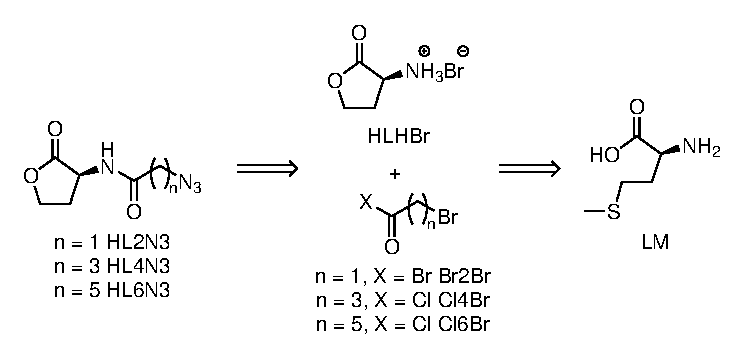
\includegraphics[scale=1]{HL246N3_retro}
		\caption{The retrosynthesis of \compound{cmpd:HL2N3}, \compound{cmpd:HL4N3} and \compound{cmpd:HL6N3}. \label{sch:HL246N3_retro}}
	\end{center}
\end{scheme}

%\begin{scheme}[H]
%	\begin{center}
%		\schemeref[LM]{cmpd:LM}
%		\schemeref[HLHBr]{cmpd:HLHBr}
%		\schemeref[Br2Br]{cmpd:Br2Br}
%		\schemeref[HL2Br]{cmpd:HL2Br}
%		\schemeref[HL2N3]{cmpd:HL2N3}
%		\includegraphics[scale=1]{HL2N3_retro}
%		\caption{The retrosynthesis of \compound{cmpd:HL2N3} \label{sch:HL2N3_retro}}
%	\end{center}
%\end{scheme}

\subsubsection{Synthesis of C$_4$-HSL derivatives \compound{cmpd:HL2N3}, \compound{cmpd:HL4N3} and \compound{cmpd:HL6N3}\label{sec:HL4N3}}

Homoserine lactone HBr salt \compound{cmpd:HLHBr} was synthesised using the procedure developed by Stacey \textit{et al.} \cite{Stacy2013}, followed by conversion to the azido-C$_2$ analogue \compound{cmpd:HL2N3} (see \ref{sch:HL2N3_synth}). Attempts to convert homoserine lactone \compound{cmpd:LM} to the azido-C$_4$ analogue using 4-bromobutyryl chloride \compound{cmpd:Cl4Br} produced a complex mixture of products. This is likely to be because the S$_N$2 reaction where the azide anion displaces bromine is slower as the bromine atom being displaced is no longer next to a carbonyl group. Hence, this allows more side reactions to occur instead of the desired reaction. It was therefore decided that the conversion should be carried out as a two-step process, where a bromoacyl chain is first installed, followed by the S$_N$2 reaction with \ce{NaN3} (see \ref{sch:HL46N3_synth}). 

Reaction of the homoserine lactone HBr salt \compound{cmpd:HLHBr} with 4-bromobutyryl chloride \compound{cmpd:Cl4Br} or 6-bromohexanoyl chloride \compound{cmpd:Cl6Br} produced bromo-C$_4$ analogue \compound{cmpd:HL4Br} or bromo-C$_6$ analogue \compound{cmpd:HL6Br} respectively. Heating with \ce{NaN3} in DMF converted bromo-C$_6$ analogue \compound{cmpd:HL6Br} to azido-C$_6$ analogue \compound{cmpd:HL6N3}\cite{Baker2012}. It is hoped that the same conditions can be used to convert bromo-C$_4$ analogue \compound{cmpd:HL4Br} to azido-C$_4$ analogue \compound{cmpd:HL4N3} and this will be attempted shortly.\todo{got from Bin Yu}

\begin{scheme}[H]
	\begin{center}
		\schemeref[LM]{cmpd:LM}
		\schemeref[HLHBr]{cmpd:HLHBr}
		\schemeref[Br2Br]{cmpd:Br2Br}
		\schemeref[HL2N3]{cmpd:HL2N3}
		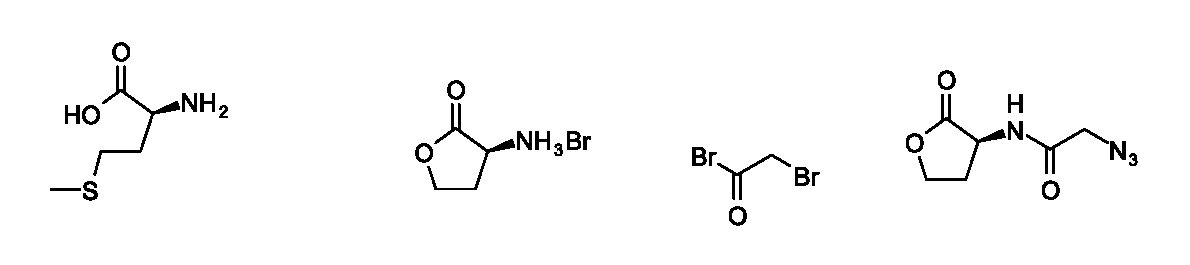
\includegraphics[scale=1]{HL2N3_synth}
		\caption{The synthesis of \compound{cmpd:HL2N3}.
		a) Bromoacetic acid, \textit{i}-PrOH:\ce{H2O}:AcOH (5:5:2), r.t., 18 h, 41 \%.
		b) \ce{NaN3}, \ce{NaHCO3}, \ce{H2O}/\ce{CH2Cl2}, r.t., 18 h, 41 \%.
		\label{sch:HL2N3_synth}}
	\end{center}
\end{scheme}
%
%\begin{scheme}[H]
%	\begin{center}
%		\schemeref[LM]{cmpd:LM}
%		\schemeref[HLHBr]{cmpd:HLHBr}
%		\schemeref[Cl4Br]{cmpd:Cl4Br}
%		\schemeref[Cl6Br]{cmpd:Cl6Br}
%		\schemeref[HL4Br]{cmpd:HL4Br}
%		\schemeref[HL6Br]{cmpd:HL6Br}
%		\schemeref[HL4N3]{cmpd:HL4N3}
%		\schemeref[HL6N3]{cmpd:HL6N3}
%		\includegraphics[scale=1]{HL46N3_retro}
%		\caption{The retrosynthesis of \compound{cmpd:HL4N3} and \compound{cmpd:HL6N3} \label{sch:HL46N3_retro}}
%	\end{center}
%\end{scheme}

\begin{scheme}[H]
	\begin{center}
		\schemeref[LM]{cmpd:LM}
		\schemeref[HLHBr]{cmpd:HLHBr}
		\schemeref[Cl4Br]{cmpd:Cl4Br}
		\schemeref[Cl6Br]{cmpd:Cl6Br}
		\schemeref[HL4Br]{cmpd:HL4Br}
		\schemeref[HL6Br]{cmpd:HL6Br}
		\schemeref[HL4N3]{cmpd:HL4N3}
		\schemeref[HL6N3]{cmpd:HL6N3}
		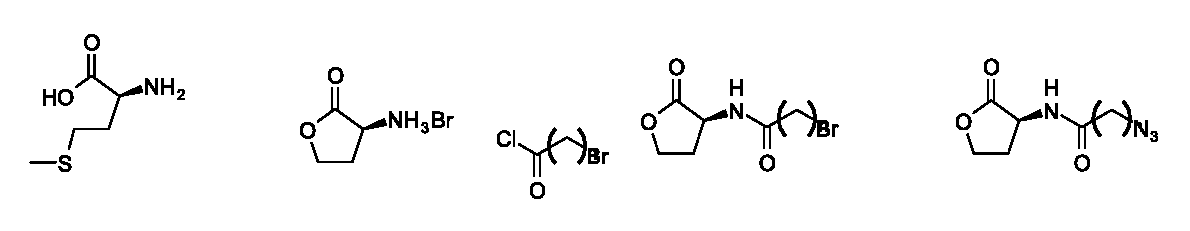
\includegraphics[scale=1]{HL46N3_synth}
		\caption{The synthesis of \compound{cmpd:HL4N3} and \compound{cmpd:HL6N3}.
		a) Bromoacetic acid, \textit{i}-PrOH:\ce{H2O}:AcOH (5:5:2), r.t, 18 h, 41 \%.
		b) \ce{NaHCO3}, \ce{H2O}/\ce{CH2Cl2}, r.t., 18 h, \compound{cmpd:HL4Br} : 80 \%, \compound{cmpd:HL6Br} : 66 \%.
		c) \ce{NaN3}, DMF, 100 $^{\circ}$C, 5 h, \compound{cmpd:HL6N3} : 56 \%.
		\label{sch:HL46N3_synth}}
	\end{center}
\end{scheme}